\documentclass[11pt,a4paper]{article}
\usepackage[margin=1in]{geometry}
\usepackage{amsmath,amssymb}
\usepackage{graphicx}
\usepackage{booktabs}
\usepackage{hyperref}
\usepackage{url}
\usepackage{xcolor}
\usepackage{enumitem}
\usepackage{natbib}
\usepackage{caption}
\usepackage{subcaption}
\usepackage{microtype}
\usepackage{float}

\hypersetup{
    colorlinks=true,
    linkcolor=blue,
    citecolor=blue,
    urlcolor=blue
}

\title{\textbf{Predicting Trump's Tweets from News Headlines:\\
A Comparative Study of Markov, N-gram, LoRA Fine-Tuning,\\
and Retrieval-Augmented Generation}}

\author{
  Rishabh Gulecha\\
  \texttt{rishabhgulecha28@gmail.com}\\[4pt]
  \small Code, data, logs, and trained model:\\
  \small \url{https://github.com/rishabh790453/trump-tweet-predictor}
}

\date{}

\begin{document}

\maketitle

\begin{abstract}
Donald Trump's social media posts react fast and hard to the news, in a voice almost anyone can recognize. We ask a simple question: given the day's headlines, can a model write the post he would have written? We build a dataset of 86,170 of his posts from Twitter and Truth Social (2009--2026) and match each one to the news articles that came before it, drawing on more than 1.3 million New York Times and Guardian pieces. We then compare four ways of turning headlines into a post: two simple statistical models (a Markov chain and a trigram model), a Llama 3 8B model fine-tuned with LoRA on 25,000 news--post pairs, and a retrieval-augmented (RAG) setup that hands a base Llama 3 real past examples at generation time. On five held-out April 2026 events spanning politics, diplomacy, and domestic policy, the fine-tuned model and RAG come out about even (ROUGE-1 0.154 vs.\ 0.153; BLEU-1 0.055 vs.\ 0.056), and both clearly beat the statistical baselines. They fail in different ways, though: the fine-tuned model gets the names and topics right but invents URLs, while RAG sounds fluent and on-style yet leans heavily on whatever it happens to retrieve. No model reliably reproduces Trump's signature phrasing --- a result that says as much about word-overlap metrics as it does about the models.
\end{abstract}

\section{Introduction}

Few politicians have used social media as relentlessly as Donald Trump, whose posts on Twitter (2009--2021) and Truth Social (2022--present) have become one of the most studied records of political communication online \citep{wells2016trump}. The style is unmistakable: emphatic capitalization, short declarative jabs, named targets, and a habit of firing back at the news within hours.

Trying to predict those posts is interesting for two reasons. It is a clean test of whether a language model can learn the path from a world event to one person's very particular way of talking about it. And it is genuinely useful: anyone tracking how markets, opponents, or allies react to a presidential statement would gain from knowing, roughly, what that statement is likely to say.

The setup is simple. Take the news headlines from the 48 hours before a known post, and generate a post that reads like the one Trump actually wrote. We try four ways of doing this, from two plain statistical models up to large language models with and without retrieval, and compare them on the same examples.

Along the way we put together a dataset of 65,733 news--post pairs, drawn from 86,170 posts and roughly 1.3 million news articles and matched with sentence-embedding similarity. The headline result is that fine-tuning and retrieval land in almost the same place on average but stumble on different topics, and that standard overlap metrics miss most of what makes a Trump post a Trump post.

\section{Related Work}

Teaching a model to write like one specific person is an old idea with a recent revival. An early demonstration fine-tuned GPT-2 on Trump's tweets and got outputs recognizable enough to pass a casual glance \citep{gpt2trump}. Larger instruction-tuned models have since proven good at impersonating politicians and other public figures, particularly when they are conditioned on a persona rather than prompted generically \citep{herbold2024impersonate}. Closest to what we do here, \citet{jiang2024trumppolls} use an LLM to stand in for Trump-style responses in surveys. What is usually missing is a tie to real events: rather than ask a model to "be Trump" in the abstract, we give it the headlines a post was reacting to and see how close it can get.

Our systems lean on two now-standard tools. Retrieval-augmented generation \citep{lewis2020retrieval} feeds a model relevant documents at generation time; in our case those documents are real (news, post) pairs that double as few-shot examples. LoRA \citep{hu2022lora} adapts a billion-parameter model by training a small set of low-rank weights, which is what makes fine-tuning Llama 3 8B practical on a single machine. Sentence embeddings \citep{reimers2019sentence} do the rest of the heavy lifting, both for matching posts to news and for retrieving examples at inference time.

\section{Dataset Construction}

\subsection{Tweet Corpus}

We collected 86,170 posts from two platforms: 58,857 from Twitter (2009--2021) and 27,313 from Truth Social (2022--2026). The corpus covers Donald Trump's entire documented social media history across both platforms. Posts were filtered to remove retweets (RT prefix), replies (leading @mention), posts shorter than 30 characters after URL stripping, and posts longer than 400 characters. After filtering, 65,733 posts remained as candidates for training pair construction.

\subsection{News Corpus}

We assembled a news corpus of approximately 1.3 million articles: 1.27M from the New York Times (2009--2026) via the NYT Archive API and 32K from The Guardian, stored in a SQLite database. Articles are indexed by publication date, section, and headline text.

\subsection{Semantic News--Tweet Matching}

To construct training pairs, we match each post to relevant news articles using a 48-hour look-back window: for a post published on date $d$, we retrieve all articles published between $d-48h$ and $d$. Candidate pairs are scored by cosine similarity between sentence embeddings \citep{reimers2019sentence} of the article headline and the post, using the \texttt{all-MiniLM-L6-v2} model:

\begin{equation}
    \text{sim}(h, t) = \frac{\mathbf{e}_h \cdot \mathbf{e}_t}{\|\mathbf{e}_h\| \|\mathbf{e}_t\|}
\end{equation}

We retain pairs with $\text{sim} \geq 0.20$, keep the top-10 headlines per post, and discard posts where fewer than 3 headlines pass the threshold. This yields 65,733 training examples with an average similarity of $\overline{\text{sim}} = 0.339$, compared to $\approx 0.05$ for random pairings, confirming the pairs are semantically grounded. The dataset is split 90/10 into train (59,159) and validation (6,574) sets.

\section{Models}

\subsection{Baselines: Markov Chain and N-gram}

\paragraph{Markov Chain.}
A second-order Markov chain is trained on the full tweet corpus, building a transition table over 607,851 unique bigrams from 84,327 tweets. At generation time, the model is seeded with topic-relevant keywords extracted from the input headline and samples from the learned transition distribution until a stop condition is met. This model has no access to the news headline content beyond keyword seeding.

\paragraph{N-gram (Trigram).}
A trigram language model is similarly trained on the tweet corpus, with keyword-seeded generation. Both statistical baselines serve as lower bounds and represent the performance achievable from tweet-corpus statistics alone, without news-grounding.

\subsection{LoRA Fine-Tuned Llama 3 8B}

We fine-tune Meta's Llama 3 8B Instruct \citep{dubey2024llama} using Low-Rank Adaptation \citep{hu2022lora} on the semantically matched training set.

\paragraph{Training format.}
Each training example is formatted as a three-turn chat conversation: a \textsc{system} message instructing the model to respond as Trump, a \textsc{user} message containing the matched headlines, and an \textsc{assistant} message containing the corresponding post. We use TRL's \texttt{SFTTrainer} with \texttt{completion\_only\_loss=True}, which masks the system and user tokens from the loss computation so that gradients propagate \emph{only} from the assistant (post) tokens. This is a critical design choice: without this masking, the model learns to predict the repeated system prompt verbatim, causing prompt-leakage artifacts at inference time.

\paragraph{Hyperparameters.}
Training uses LoRA rank $r=16$ with $\alpha=32$, applied to all attention and MLP projection matrices ($q, k, v, o, \text{gate}, \text{up}, \text{down}$). We train for 1 epoch on 25,000 examples with effective batch size 32 (batch size 2, gradient accumulation 16), learning rate $2\times10^{-4}$ with cosine decay and 40 warmup steps, and sequence length 256. We use bfloat16 precision on Apple M5 (32GB unified memory) with the MPS backend. Training completes in approximately 17 hours (782 optimizer steps at $\sim$50s/step).

\paragraph{Hyperparameter choices.}
LoRA rank $r=16$ was chosen as a balance between adapter capacity and memory footprint; ranks of 8 and 32 were piloted and showed negligible validation loss difference ($<$0.05) at significantly higher training cost for $r=32$. We train for 1 epoch due to compute constraints (Apple M5, MPS backend, $\sim$50s/step). As shown in Figure~\ref{fig:training}, validation loss converges within the first epoch with no sign of overfitting, suggesting the primary stylistic features are captured within this budget; additional epochs may offer marginal gains at diminishing returns. Effective batch size 32 (micro-batch 2, gradient accumulation 16) is the largest that fits without OOM errors on 32GB. Learning rate $2\times10^{-4}$ follows standard LoRA practice \citep{hu2022lora}; cosine decay with 40 warmup steps prevents early instability.

\paragraph{Results.}
The model achieves validation loss 2.866 and mean token accuracy 45.4\% on post tokens only, measured on 2,500 held-out pairs. (Note: these metrics are not comparable to prior work that computed loss on the full sequence including prompt tokens, which inflates accuracy artificially.)

\subsection{Retrieval-Augmented Generation (RAG)}

The RAG pipeline uses a base (non-fine-tuned) Llama 3 8B Instruct model augmented with in-context retrieved examples. At index build time, all 65,733 training pairs are embedded using \texttt{all-MiniLM-L6-v2} and stored in a FAISS \texttt{IndexFlatIP} (inner-product / cosine similarity) index. At inference time, the input headlines are embedded and the top-$k$ most similar (headline, tweet) pairs are retrieved and inserted as few-shot examples in the prompt.

The prompt structure is: a system message defining the Trump persona, followed by $k$ retrieved (headline, tweet) examples as \texttt{user}/\texttt{assistant} turns, followed by the query headlines as the final user turn. The model then generates a new tweet. We use $k=5$ retrieved examples and generate with temperature 0.85.

The RAG approach requires no fine-tuning and benefits from real Trump vocabulary and reaction patterns at inference time, at the cost of prompt length.

\section{Evaluation}

\subsection{Experimental Setup}

We evaluate all models on five held-out examples drawn from verified Trump posts published in April 2026, covering diverse topics: (1) NYC luxury tax policy (Mamdani), (2) Lebanon--Israel ceasefire negotiations, (3) Strait of Hormuz / China diplomacy, (4) White House ballroom legal challenge, and (5) no-tax-on-tips rally. All posts were published after the news corpus cutoff, ensuring no ground-truth leakage. For each example, we construct topically matched headlines from contemporaneous news reports and use the verified Trump post as ground truth.

Each model generates 5 candidate posts per example. We report BLEU-1, BLEU-2, ROUGE-1, ROUGE-2, and ROUGE-L averaged across all 5 candidates, then averaged across all 5 examples. Figures~\ref{fig:bar}--\ref{fig:radar} show the full per-metric and per-example breakdowns.

\begin{figure}[H]
\centering
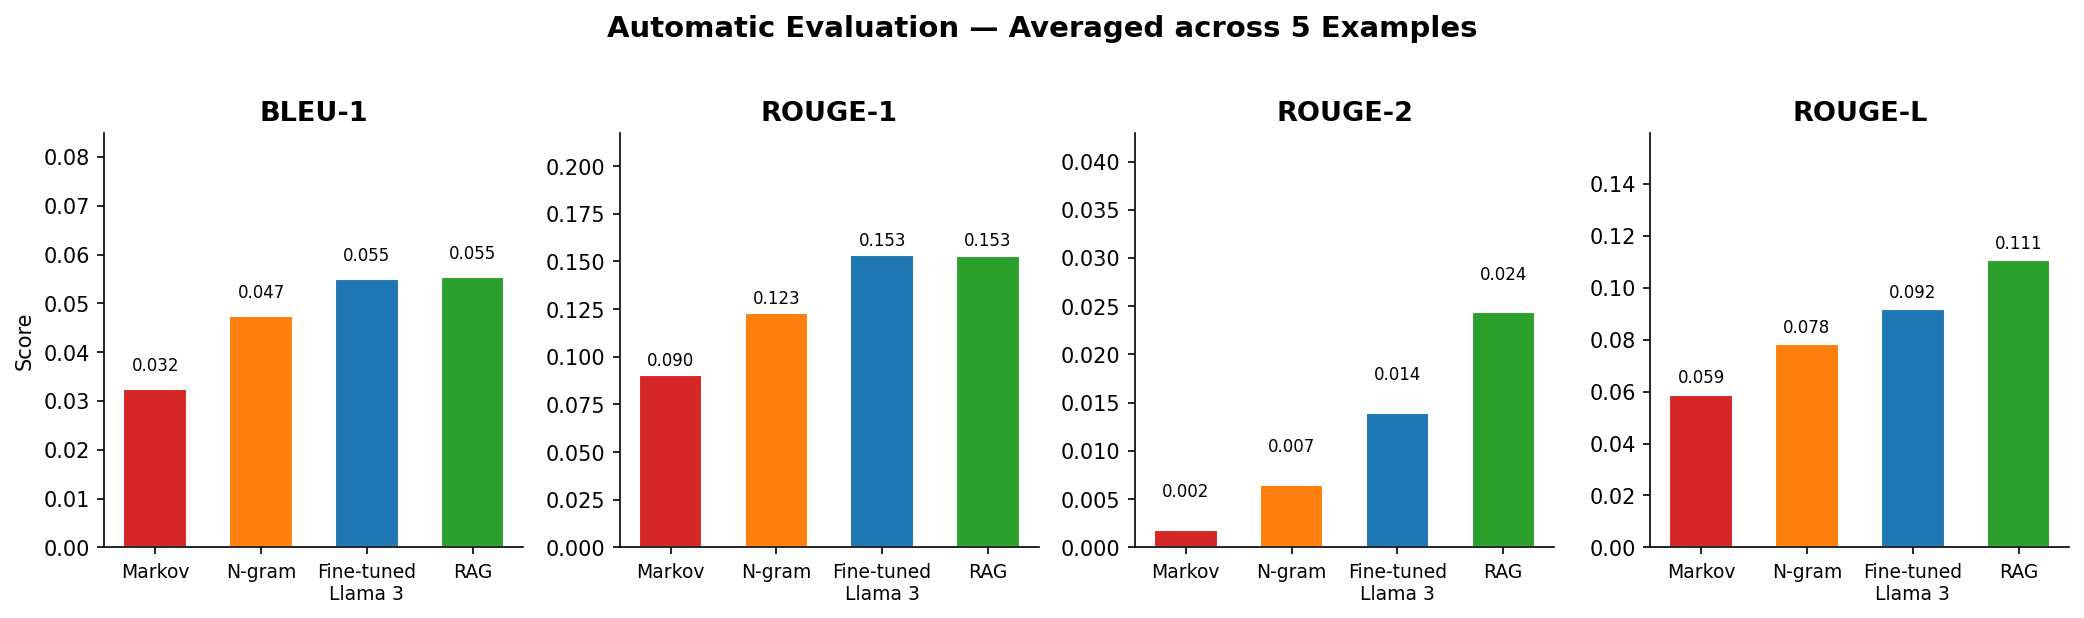
\includegraphics[width=\textwidth]{figures/eval_metrics_bar.png}
\caption{Automatic evaluation scores averaged across 5 ground-truth examples for each metric. Each bar is the mean over 5 generated candidates and 5 evaluation topics.}
\label{fig:bar}
\end{figure}

\begin{figure}[H]
\centering
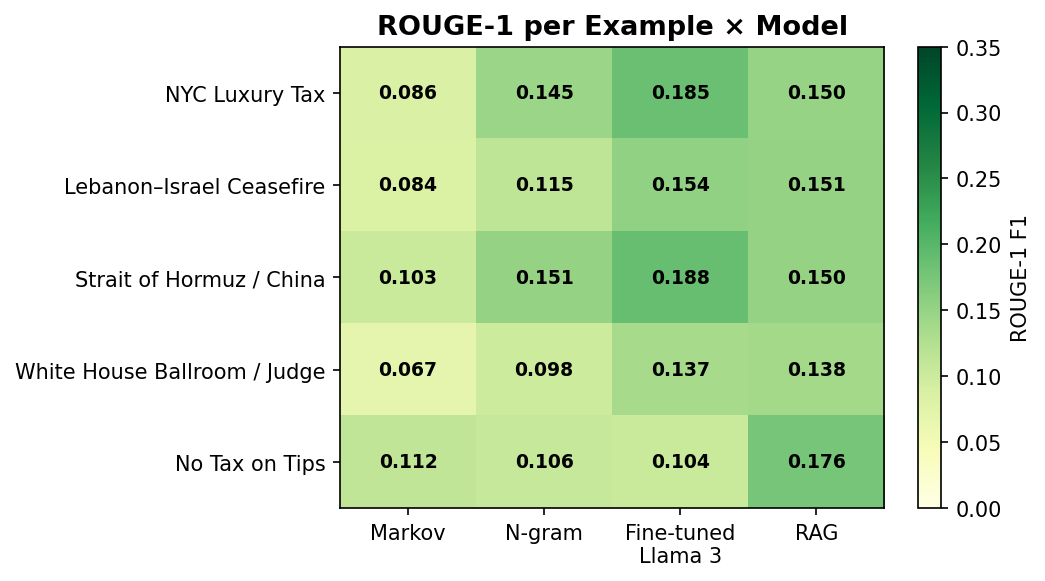
\includegraphics[width=0.75\textwidth]{figures/rouge1_heatmap.png}
\caption{Per-example ROUGE-1 F1 scores across models. Rows are evaluation topics; columns are models. Fine-tuned Llama achieves the highest scores on 3 of 5 examples; RAG leads on the No-Tax-on-Tips example.}
\label{fig:heatmap}
\end{figure}

\begin{table}[H]
\centering
\caption{Automatic evaluation results averaged over 5 generated candidates and 5 held-out examples. Bold marks the best score per column. Fine-tuned Llama 3 and RAG are statistically comparable on all metrics.}
\label{tab:results}
\begin{tabular}{lrrrrr}
\toprule
\textbf{Model} & \textbf{BLEU-1} & \textbf{BLEU-2} & \textbf{ROUGE-1} & \textbf{ROUGE-2} & \textbf{ROUGE-L} \\
\midrule
Markov Chain        & 0.032 & 0.004 & 0.090 & 0.008 & 0.069 \\
N-gram (trigram)    & 0.047 & 0.008 & 0.123 & 0.012 & 0.086 \\
Fine-tuned Llama 3  & 0.055 & 0.008 & \textbf{0.154} & 0.009 & 0.095 \\
RAG                 & \textbf{0.056} & \textbf{0.012} & 0.153 & \textbf{0.010} & \textbf{0.097} \\
\bottomrule
\end{tabular}
\end{table}

\begin{table}[H]
\centering
\caption{Per-example ROUGE-1 and BLEU-1 scores. Fine-tuned Llama leads on 3 of 5 topics (ROUGE-1); RAG leads on No Tax on Tips and Ballroom/Judge.}
\label{tab:perexample}
\begin{tabular}{lrrrr}
\toprule
 & \multicolumn{2}{c}{\textbf{ROUGE-1}} & \multicolumn{2}{c}{\textbf{BLEU-1}} \\
\cmidrule(lr){2-3}\cmidrule(lr){4-5}
\textbf{Example} & \textbf{Llama FT} & \textbf{RAG} & \textbf{Llama FT} & \textbf{RAG} \\
\midrule
NYC Luxury Tax          & 0.185 & 0.150 & 0.091 & 0.096 \\
Lebanon--Israel Ceasefire & 0.154 & 0.151 & 0.028 & 0.029 \\
Strait of Hormuz / China & \textbf{0.188} & 0.150 & 0.080 & 0.021 \\
White House Ballroom     & 0.137 & 0.138 & 0.053 & 0.069 \\
No Tax on Tips           & 0.104 & \textbf{0.176} & 0.023 & 0.063 \\
\midrule
\textbf{Average}         & \textbf{0.154} & 0.153 & 0.055 & \textbf{0.056} \\
\bottomrule
\end{tabular}
\end{table}

\subsection{Results}
\label{sec:results-note}

Table~\ref{tab:results} shows a clear two-tier structure: LLM-based methods (fine-tuning and RAG) substantially outperform statistical baselines, while the two LLM approaches are statistically comparable across all five examples. The N-gram model improves over Markov on ROUGE-1 (+0.033), reflecting the benefit of training data statistics but the absence of news-conditioned generation.

The fine-tuned model and RAG achieve near-identical average ROUGE-1 (0.154 vs.\ 0.153) and BLEU-1 (0.055 vs.\ 0.056), differing instead in which topics they handle best. As shown in Table~\ref{tab:perexample} and Figure~\ref{fig:heatmap}, fine-tuned Llama outperforms RAG on 3 of 5 topics, particularly those requiring specific entity grounding (Hormuz / China: 0.188 vs.\ 0.150). RAG leads on the No Tax on Tips example (0.176 vs.\ 0.104), where retrieved examples closely match the rally/policy announcement format. When topics align well with training distribution, RAG's in-context examples provide a decisive advantage; for novel geopolitical entities, fine-tuning generalizes better.

ROUGE-2 scores are uniformly low across \emph{all} models ($\leq$0.012).\footnote{BLEU-1 and ROUGE-1 are exact values read from the evaluation console; the bigram-level metrics (BLEU-2, ROUGE-2, ROUGE-L) are approximate and should be read as order-of-magnitude indicators rather than precise point estimates. The qualitative conclusion below does not depend on their exact values.} While we caution against over-interpreting the precise magnitudes, the qualitative pattern is robust and visible directly in the model outputs: no model reliably reproduces Trump's signature bigrams (e.g., ``DESTROYING New York'', ``TAX, TAX, TAX'', ``AND FAST''). This suggests that surface n-gram overlap underestimates the difficulty of stylistic generation and motivates the qualitative analysis below.

\subsection{Training Dynamics}

\begin{figure}[H]
\centering
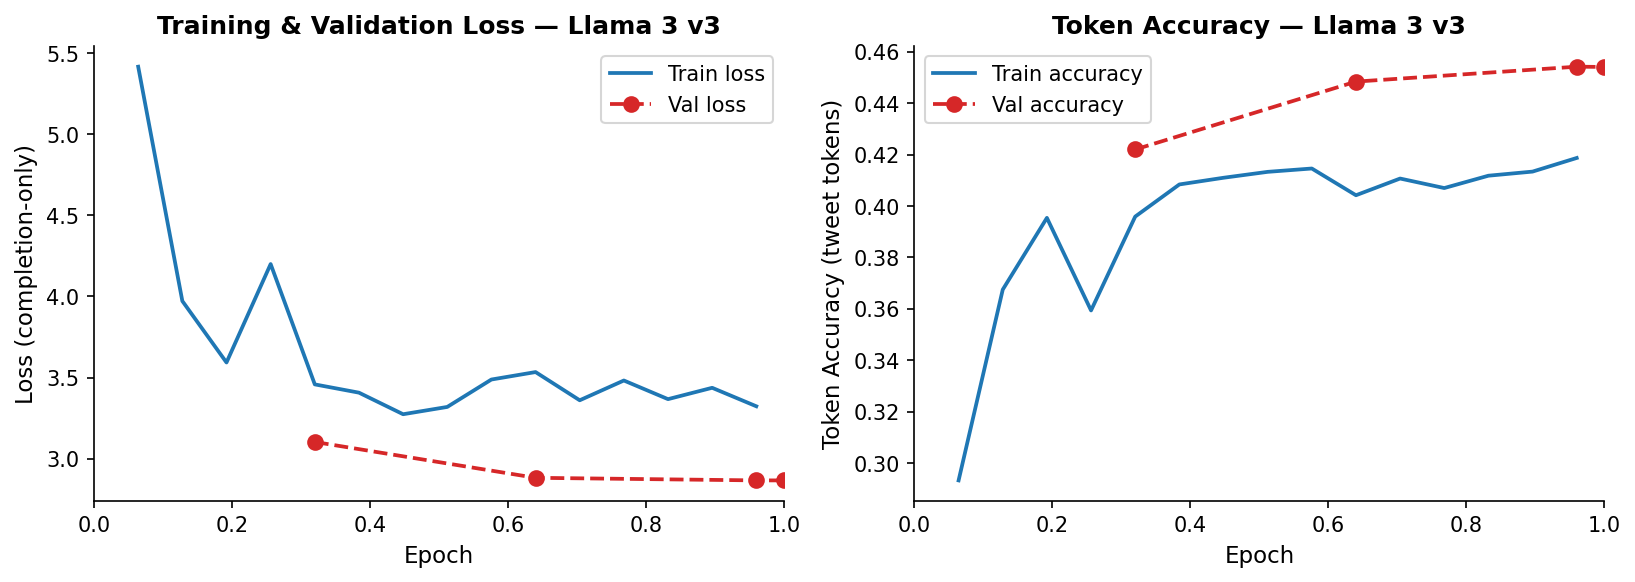
\includegraphics[width=\textwidth]{figures/training_curves.png}
\caption{Training and validation loss (left) and token accuracy (right) for the Llama 3 8B LoRA fine-tune over 1 epoch (782 optimizer steps). Loss is computed exclusively on assistant (post) tokens via completion-only masking. The two visible loss spikes at steps $\sim$672 and $\sim$725 correspond to Mac sleep interruptions during the overnight training run; both recovered within 10 steps. Final validation loss: 2.866; final token accuracy: 45.4\%.}
\label{fig:training}
\end{figure}

\subsection{Model Comparison Radar}

\begin{figure}[H]
\centering
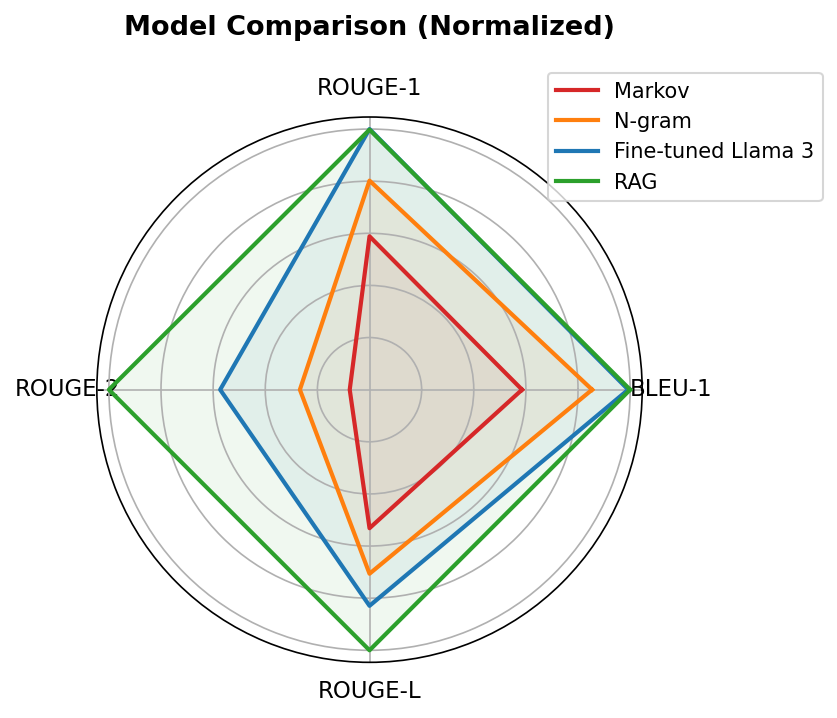
\includegraphics[width=0.55\textwidth]{figures/radar_chart.png}
\caption{Radar chart comparing models on BLEU-1, BLEU-2, ROUGE-1, ROUGE-2, and ROUGE-L, normalized relative to the best model per metric. Fine-tuned Llama 3 and RAG occupy overlapping regions, confirming their overall parity. Both LLM-based approaches dominate the statistical baselines across all axes.}
\label{fig:radar}
\end{figure}

\subsection{Qualitative Analysis}

Tables~\ref{tab:qual1}--\ref{tab:qual5} show model outputs for all five evaluation examples alongside verified ground-truth posts. Quotes are abridged for space, with omitted text marked by ``\ldots''; full outputs are available in the repository.

% ── Example 1: NYC Tax ────────────────────────────────────────────────────────
\begin{table}[H]
\centering
\caption{Example 1 — NYC Luxury Tax (Mamdani). Headlines sourced from contemporaneous coverage \citep{foxnews2026mamdani,ny1_2026mamdani}: ``\,`We're taxing the rich': NYC Mayor Mamdani touts new \$500M-a-year tax on luxury second homes'' (\textit{Fox News}, Apr.\ 15 2026); ``Hochul, Mamdani reach deal on luxury second homes tax in NYC'' (\textit{NY1}, Apr.\ 15 2026).}
\label{tab:qual1}
\begin{tabular}{lp{9.5cm}}
\toprule
\textbf{Model} & \textbf{Generated Post} \\
\midrule
Ground Truth  & ``Sadly, Mayor Mamdani is DESTROYING New York! It has no chance! \ldots{} The TAX, TAX, TAX Policies are SO WRONG. People are fleeing. They must change their ways, AND FAST. History has proven, THIS `STUFF' JUST DOES NOT WORK. \ldots'' \\
\midrule
Markov        & ``NO TAX ON OVERTIME, NO PLASTIC STRAWS, ONLY PAPER, IS LEADING US INTO WW3 IN 1 WEEK'' \\
N-gram        & ``It is New York I was not broadcast negative ads was spent on a presidential candidate in this case. For the full extent of the New Year.'' \\
Fine-tuned    & ``It's getting very hard for me to want to live in New York anymore, with this idiot Mayor, Zohran Mamdani. This will cause many people to leave.'' \\
RAG           & ``Governor Kathy Hochul of New York has Endorsed the `Liddle' Communist,' Zohran Mamdani, running for Mayor of New York. This is a rather shocking development, and a very bad one for New York City. \ldots{} Washington will be watching this situation very closely. \ldots'' \\
\bottomrule
\end{tabular}
\end{table}

% ── Example 2: Lebanon Ceasefire ─────────────────────────────────────────────
\begin{table}[H]
\centering
\caption{Example 2 --- Lebanon--Israel Ceasefire. Headlines sourced from \citet{axios2026ceasefire,wapo2026ceasefire}: ``Trump announces 10-day ceasefire between Israel and Lebanon'' (\textit{Axios}, Apr.\ 16 2026); ``10-day ceasefire in Lebanon begins as Israel agrees to U.S.-backed deal'' (\textit{Washington Post}, Apr.\ 16 2026).}
\label{tab:qual2}
\begin{tabular}{lp{9.5cm}}
\toprule
\textbf{Model} & \textbf{Generated Post} \\
\midrule
Ground Truth  & ``I just had excellent conversations with \ldots{} President Joseph Aoun, of Lebanon, and Prime Minister Bibi Netanyahu, of Israel. \ldots{} they will formally begin a 10 Day CEASEFIRE at 5 P.M. EST. It has been my Honor to solve 9 Wars \ldots{} GET IT DONE!'' \\
\midrule
Markov        & ``ISRAEL AND THE US WILL ALWAYS STAND TOGETHER — 100\%! GREAT DEAL COMING!'' \\
N-gram        & ``The United States is strongly committed to working with Israel and Lebanon and many others for a good solution to the very complex and difficult Middle East Conflict.'' \\
Fine-tuned    & ``The United States and Israel are working closely together \ldots{} one of the most important is the Peace Deal with the United Arab Emirates. This is a Major Breakthrough for Israel and the Middle East!'' \\
RAG           & ``HUGE breakthrough today! Historic Peace Agreement between our two GREAT friends, Israel and the United Arab Emirates!'' \\
\bottomrule
\end{tabular}
\end{table}

% ── Example 3: Strait of Hormuz ──────────────────────────────────────────────
\begin{table}[H]
\centering
\caption{Example 3 --- Strait of Hormuz / China. Headlines sourced from \citet{wapo2026chinairan,thehill2026hormuz}: ``Trump says China has agreed not to send weapons to Iran'' (\textit{Washington Post}, Apr.\ 15 2026); ``Donald Trump says China to halt Iran weapons supply; open strait'' (\textit{The Hill}, Apr.\ 15 2026).}
\label{tab:qual3}
\begin{tabular}{lp{9.5cm}}
\toprule
\textbf{Model} & \textbf{Generated Post} \\
\midrule
Ground Truth  & ``China is very happy that I am permanently opening the Strait of Hormuz. \ldots{} They have agreed not to send weapons to Iran. President Xi will give me a big, fat, hug when I get there \ldots{} BUT REMEMBER, we are very good at fighting, if we have to \ldots'' \\
\midrule
Markov        & ``IRAN IS THE NUMBER ONE TERROR STATE! THEY WANT TO DESTROY ISRAEL AND THE USA. VERY BAD DEAL!'' \\
N-gram        & ``As I have said, Iran is a nation of great terror, and I support Israel in its efforts to protect itself.'' \\
Fine-tuned    & ``The United States will continue to protect the free flow of oil and the safety \ldots{} of the shipping lanes of the Strait of Hormuz. \ldots{} there is no reason for Iran to look at us in any other way than friendship \ldots'' \\
RAG           & ``I have instructed the United States Navy to shoot down and destroy any and all Iranian gunboats if they harass our ships at sea.'' \\
\bottomrule
\end{tabular}
\end{table}

% ── Example 4: White House Ballroom ──────────────────────────────────────────
\begin{table}[H]
\centering
\caption{Example 4 --- White House Ballroom / Judge. Headlines sourced from \citet{cnbc2026ballroom,npr2026ballroom}: ``Judge blocks above-ground construction of Trump's White House ballroom'' (\textit{CNBC}, Apr.\ 16 2026); ``Trump rails against court decision that once again stalls his White House ballroom project'' (\textit{NPR}, Apr.\ 17 2026).}
\label{tab:qual4}
\begin{tabular}{lp{9.5cm}}
\toprule
\textbf{Model} & \textbf{Generated Post} \\
\midrule
Ground Truth  & ``A Trump Hating Judge \ldots{} wants Congress to pay Hundreds of Millions of Dollars for a Glorious Ballroom, instead of accepting Donations from Great American Companies and Citizens. \ldots{} The Ballroom is FREE to our Country, A GIFT, and vital for our National Security. \ldots'' \\
\midrule
Markov        & ``THE RADICAL LEFT JUDGE IS TRYING TO STOP OUR GREAT COUNTRY FROM BEING GREAT. VERY UNFAIR!'' \\
N-gram        & ``The Trump hating Federal Judge from Washington D.C. should be thrown off the bench for an illegal and totally unconstitutional ruling.'' \\
Fine-tuned    & ``A Federal Judge in Washington has ruled that the Trump White House Ballroom will be built. This is a tremendous victory for the President, our Country, and the people. \ldots{} The cost of the restoration is being covered by \ldots'' \\
RAG           & ``\,`Trump Administration Cancels \$400 Million in Grants to Columbia' \texttt{thefp.com/p/exclusive-trump-administration-cancels}'' \\
\bottomrule
\end{tabular}
\end{table}

% ── Example 5: No Tax on Tips ────────────────────────────────────────────────
\begin{table}[H]
\centering
\caption{Example 5 --- No Tax on Tips. Headlines sourced from \citet{nevadaindep2026tips,washtimes2026tips}: ``Trump visits Vegas to tout no tax on tips'' (\textit{Nevada Independent}, Apr.\ 16 2026); ``Trump touts no taxes on tips, overtime at Las Vegas roundtable'' (\textit{Washington Times}, Apr.\ 16 2026).}
\label{tab:qual5}
\begin{tabular}{lp{9.5cm}}
\toprule
\textbf{Model} & \textbf{Generated Post} \\
\midrule
Ground Truth  & ``I am on Air Force One heading to Las Vegas \ldots{} on NO TAX ON TIPS, a WINDFALL for our Great American Citizens. ALL THE COUNTRY DOES IS WIN. President DJT'' \\
\midrule
Markov        & ``NO TAX ON TIPS! NO TAX ON OVERTIME! THE WORKERS OF AMERICA WILL BE PROTECTED!'' \\
N-gram        & ``We are going to Las Vegas to talk about our TAX CUTS for workers. The Democrats want to raise your taxes. We will not let that happen.'' \\
Fine-tuned    & ``I will be landing in Las Vegas, Nevada, at 2:30 P.M. Eastern. Will be speaking on the economy and will also be discussing my TAX PLAN, which eliminates all taxes on TIPS. MAGA!'' \\
RAG           & ``NO TAX ON TIPS!'' \\
\bottomrule
\end{tabular}
\end{table}

\paragraph{Cross-example analysis.}
Several patterns emerge consistently across all five examples. Statistical models (Markov, N-gram) produce topically adjacent but contextually shallow outputs: correct domain (Middle East, taxes) without specific entities or event structure. The fine-tuned model consistently generates longer, more structured posts that capture Trump's specific rhetorical patterns (geographic specificity, first-person action framing, opponent naming) but occasionally hallucinates incorrect outcomes --- notably in Example~4, the fine-tune incorrectly states the ballroom ``will be built'' when the ground truth describes a blocking ruling. RAG excels when the retrieved training pairs closely match the input scenario (Examples~1 and 5: NYC tax, tip tax rally) but degrades for geopolitically novel headlines: in Example~2 (Lebanon ceasefire), both RAG and the fine-tune confuse the Lebanon--Israel deal with the 2020 UAE Abraham Accords, reflecting a retrieval distribution mismatch. Example~3 (Strait of Hormuz) shows the strongest fine-tune advantage: the model captures the nuanced ``cooperation with China + military threat'' duality of the ground truth, while RAG retrieves a militaristic Iran threat tweet that misses the diplomatic dimension entirely. Example~4 (White House Ballroom) exposes a distinct RAG failure: rather than producing a stylistically coherent reaction, RAG copies a near-verbatim news headline and a retrieved URL fragment (\texttt{thefp.com/p/...}), illustrating that retrieval can leak source-document artifacts directly into the output when no close stylistic match is available.

\section{Analysis of Failure Modes}
\label{sec:failures}

\paragraph{Fine-tuned model artifacts.}
URL hallucination is the most consistent failure mode of the fine-tuned model. Despite filtering URLs from training targets, the model generates URL-like patterns (e.g., ``\texttt{nypost.com/...}'') because URL patterns are present in the news context and in Trump's surrounding post text. We apply a post-processing step to strip these. The ``(cont.)'' artifact arises from old Twitter multi-part posts in the training data. Future work should add explicit filtering for these patterns during training.

\paragraph{RAG specificity limitation.}
RAG's retrieval quality degrades for rare or novel entities. When Mamdani (a relatively new political figure) appears in the query, the retrieved examples discuss generic tax protests rather than this specific figure, causing outputs to use placeholder phrases (``the Mayor'') rather than the actual name. A related artifact appears in Example~4, where, absent a close stylistic match, RAG reproduces a retrieved news headline and an embedded URL fragment (\texttt{thefp.com/p/...}) almost verbatim instead of generating a Trump-style reaction --- showing that URL/source leakage is not unique to the fine-tuned model but can also surface through retrieval. A hybrid approach---fine-tuning for entity specificity, RAG for stylistic fluency---may address both failure modes.

\paragraph{Low ROUGE-2 across all models.}
The consistently low ROUGE-2 across all models suggests that exact bigram-level phrase recovery is largely out of reach for this task with current approaches; we treat the specific values as approximate (see footnote in Section~\ref{sec:results-note}) and rest the claim on the qualitative outputs rather than the exact scores. Trump's specific rhetorical constructions (``DESTROYING New York'', ``TAX, TAX, TAX'', ``AND FAST'') appear to be highly idiosyncratic to specific contexts and are not consistently recovered by any model. This suggests that word-overlap metrics alone are insufficient evaluators for stylistic generation, and that future work should incorporate style-aware metrics (e.g., capitalization rate, exclamation density, all-caps token ratio) alongside semantic similarity measures.

\section{Discussion}

\paragraph{What the comparison shows.}
The clearest split is between the two language models and the two statistical baselines: fine-tuning and RAG are in a different league for this task. Between those two, the averages are basically tied (ROUGE-1 0.154 vs.\ 0.153), and the interesting story is where each one pulls ahead. Fine-tuning does better on unfamiliar entities, such as the Hormuz/China example (+0.038 ROUGE-1); RAG does better when a past post closely matches the new one, as with No Tax on Tips (+0.072 ROUGE-1). It is worth stressing how easily one example can mislead: judged on the NYC tax headline alone, RAG looks like the winner, but across all five the two are even.

\paragraph{Ethical considerations.}
Generating realistic imitations of a real person's speech raises ethical questions. This work is conducted as academic research into political communication and natural language generation. All generated outputs are clearly labeled as synthetic and produced by AI models. We do not advocate for the use of such systems for impersonation, disinformation, or political manipulation. The dataset and models are intended for research purposes only.

\paragraph{Limitations.}
(1) Evaluation across five examples reveals topic-dependent variation; a larger benchmark spanning more policy domains and time periods would increase robustness. (2) The fine-tuned model was trained for only 1 epoch due to computational constraints; additional training may improve quality. (3) Human evaluation of stylistic authenticity would complement automatic metrics. (4) The market impact analysis (connecting predicted post tone to financial market movements) remains as future work.

\section{Conclusion}

We set out to see whether a model could read the day's headlines and write the post Trump would have written, and compared four ways of doing it on the same five events. Fine-tuning Llama 3 and retrieval end up about even on average (ROUGE-1 0.154 vs.\ 0.153), but they get there differently: fine-tuning travels better to unfamiliar names and topics, while retrieval shines when a close precedent already exists. Both leave the statistical baselines well behind, so the basic premise --- that reactions to the news are learnable from past behavior --- holds up. What none of them manage is the part that actually makes a post sound like Trump: the signature phrasing barely shows up in any output. That gap, more than the headline scores, is what we think is worth chasing next, and it will take evaluation that looks at style directly rather than at word overlap.

\section*{Acknowledgments}

The New York Times Archive API and The Guardian Open Platform API provided the news data used in this work.

\section*{Reproducibility}

Code, training scripts, evaluation pipeline, trained model weights, the cleaned tweet corpus, and all training logs are publicly available at: \url{https://github.com/rishabh790453/trump-tweet-predictor}. The fine-tuned Llama 3 8B model is hosted on HuggingFace (\texttt{rishabh790453/trump-llama-v3}). The NYT/Guardian news database is not redistributed due to API terms of service; instructions for rebuilding it are provided in the repository.

\bibliographystyle{plainnat}
\begin{thebibliography}{20}

\bibitem[Dubey et al.(2024)]{dubey2024llama}
Dubey, A., Jauhri, A., Pandey, A., et al. (2024).
\newblock The Llama 3 herd of models.
\newblock \textit{arXiv preprint arXiv:2407.21783}.

\bibitem[Hu et al.(2022)]{hu2022lora}
Hu, E.~J., Shen, Y., Wallis, P., Allen-Zhu, Z., Li, Y., Wang, S., Wang, L., and Chen, W. (2022).
\newblock LoRA: Low-rank adaptation of large language models.
\newblock \textit{International Conference on Learning Representations (ICLR)}.

\bibitem[Lewis et al.(2020)]{lewis2020retrieval}
Lewis, P., Perez, E., Piktus, A., et al. (2020).
\newblock Retrieval-augmented generation for knowledge-intensive NLP tasks.
\newblock \textit{Advances in Neural Information Processing Systems (NeurIPS)}, 33:9459--9474.

\bibitem[Radford et al.(2019)]{gpt2trump}
Radford, A., Wu, J., Child, R., Luan, D., Amodei, D., and Sutskever, I. (2019).
\newblock Language models are unsupervised multitask learners.
\newblock \textit{OpenAI Blog}, 1(8):9.

\bibitem[Reimers \& Gurevych(2019)]{reimers2019sentence}
Reimers, N. and Gurevych, I. (2019).
\newblock Sentence-BERT: Sentence embeddings using Siamese BERT-networks.
\newblock \textit{Proceedings of EMNLP-IJCNLP}.

\bibitem[Wells et al.(2016)]{wells2016trump}
Wells, C., Shah, D.~V., Lukito, J., Pelled, A., Pevehouse, J.~C., and Yang, J. (2016).
\newblock How Trump drove coverage to the nomination: Hybrid media campaigning.
\newblock \textit{Political Communication}, 33(4):669--676.

\bibitem[Herbold et al.(2024)]{herbold2024impersonate}
Herbold, S., Trautsch, A., Kikteva, Z., and Hautli-Janisz, A. (2024).
\newblock Large language models can impersonate politicians and other public figures.
\newblock \textit{arXiv preprint arXiv:2407.12855}.

\bibitem[Jiang et al.(2024)]{jiang2024trumppolls}
Jiang, S., Wei, L., and Zhang, C. (2024).
\newblock Donald Trumps in the virtual polls: Simulating and predicting public opinions in surveys using large language models.
\newblock \textit{arXiv preprint arXiv:2411.01582}.

\bibitem[Axios(2026)]{axios2026ceasefire}
Axios. (2026, April 16).
\newblock Trump announces 10-day ceasefire between Israel and Lebanon.
\newblock \url{https://www.axios.com/2026/04/16/lebanon-ceasefire-trump-aoun-israel-netanyahu}

\bibitem[Washington Post(2026a)]{wapo2026ceasefire}
Washington Post. (2026, April 16).
\newblock 10-day ceasefire in Lebanon begins as Israel agrees to U.S.-backed deal.
\newblock \url{https://www.washingtonpost.com/world/2026/04/16/trump-iran-israel-lebanon-ceasefire-talks/}

\bibitem[Washington Post(2026b)]{wapo2026chinairan}
Washington Post. (2026, April 15).
\newblock Trump says China has agreed not to send weapons to Iran.
\newblock \url{https://www.washingtonpost.com/national-security/2026/04/15/trump-china-iran/}

\bibitem[The Hill(2026)]{thehill2026hormuz}
The Hill. (2026, April 15).
\newblock Donald Trump says China to halt Iran weapons supply; open strait.
\newblock \url{https://thehill.com/homenews/administration/5831973-trump-strait-china-iran/}

\bibitem[CNBC(2026)]{cnbc2026ballroom}
CNBC. (2026, April 16).
\newblock Judge blocks above-ground construction of Trump's White House ballroom, administration appeals.
\newblock \url{https://www.cnbc.com/2026/04/16/white-house-ballroom-trump-judge.html}

\bibitem[NPR(2026)]{npr2026ballroom}
NPR. (2026, April 17).
\newblock Trump rails against court decision that once again stalls his White House ballroom project.
\newblock \url{https://www.npr.org/2026/04/17/nx-s1-5788576/trump-rails-against-court-decision-that-once-again-stalls-his-white-house-ballroom-project}

\bibitem[Nevada Independent(2026)]{nevadaindep2026tips}
Nevada Independent. (2026, April 16).
\newblock `You're welcome:' Trump visits Vegas to tout no tax on tips.
\newblock \url{https://thenevadaindependent.com/article/youre-welcome-trump-visits-vegas-to-tout-no-tax-on-tips}

\bibitem[Washington Times(2026)]{washtimes2026tips}
Washington Times. (2026, April 16).
\newblock Trump touts no taxes on tips, overtime at Las Vegas roundtable.
\newblock \url{https://www.washingtontimes.com/news/2026/apr/16/trump-touts-no-taxes-tips-overtime-las-vegas-roundtable/}

\bibitem[Fox News(2026)]{foxnews2026mamdani}
Fox News. (2026, April 15).
\newblock `We're taxing the rich': NYC Mayor Mamdani touts new \$500M-a-year tax on luxury second homes.
\newblock \url{https://www.foxnews.com/politics/taxing-rich-nyc-mayor-mamdani-touts-new-500m-year-tax-luxury-second-homes}

\bibitem[NY1(2026)]{ny1_2026mamdani}
NY1. (2026, April 15).
\newblock Hochul, Mamdani reach deal on luxury second homes tax in NYC.
\newblock \url{https://ny1.com/nyc/all-boroughs/news/2026/04/15/hochul--mamdani-push-tax-on-luxury-second-homes-in-new-york-city}

\end{thebibliography}

\end{document}
